\documentclass{beamer}
\usepackage{tikz}
\usepackage{lstautogobble, listings, xcolor} 

\definecolor{bluekeywords}{rgb}{0.13, 0.19, 0.7}
\definecolor{goldenkeywords}{rgb}{0.67, 0.58, 0.13}
\definecolor{greencomments}{rgb}{0.1, 0.5, 0.2}
\definecolor{redstrings}{rgb}{0.8, 0.15, 0.1}
\definecolor{graynumbers}{rgb}{0.5, 0.5, 0.5}
\definecolor{subtlegray}{rgb}{0.98, 0.98, 0.98}

\lstset{
    autogobble,    
    columns=fullflexible,
    showspaces=false,
    showtabs=false,
    breaklines=true,
    showstringspaces=false,
    numbers=left,
    breakatwhitespace=true,
    escapeinside={(*@}{@*)},
    rulecolor=\color{lightgray},
    backgroundcolor=\color{subtlegray},
    commentstyle=\color{greencomments},
    keywordstyle=\color{bluekeywords},
    ndkeywordstyle=\color{goldenkeywords},
    stringstyle=\color{redstrings},
    numberstyle=\color{graynumbers},
    basicstyle=\ttfamily\linespread{1.15}\footnotesize,
    frame=tb,
    framesep=12pt,
    framexleftmargin=12pt,
    tabsize=4,
    captionpos=b
}

\lstdefinelanguage{TML}{ 
    keywords={changeto, move, goto, if, switch, while, module, accept, reject, alphabet},
    ndkeywords={left, right, tapehead, blank},
    sensitive=true,
    comment=[l]{//},
    morecomment=[s]{/*}{*/},
    morestring=[b]',
    morestring=[b]"
}

\usetikzlibrary{automata, positioning, arrows, shapes}

\title{Turing Machine Language}
\author{Pete Gautam}
\institute{University of Glasgow}

\begin{document}

    \frame{\titlepage}

    \begin{frame}{Introduction}
        \begin{itemize}
            \item Turing Machines (TM) are a model of computation.
            \item They are typically taught theoretically, i.e. pen-and-paper.
            \item Students find it hard to learn the content.
            \item Perhaps it is easier to learn as a programming language (PL)?
            \item We present a PL for TMs which abstracts TM operations but keeps tape operations concrete.
            \item We investigate whether students find this method easier than the traditional approach.
        \end{itemize}
    \end{frame}

    \begin{frame}{Turing Machines}
        \begin{itemize}
            \item Can be thought of as boolean functions on string
            \item Can be represented as a directed graph (called FSM)
            \item Has states and transitions
        \end{itemize}

        \begin{figure}[htb]
            \centering
            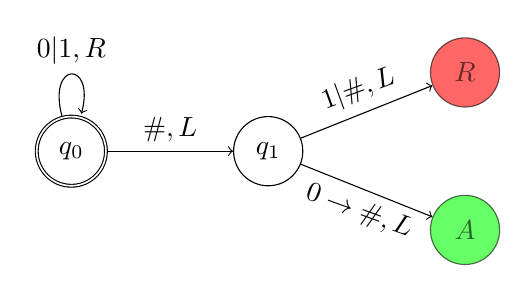
\begin{tikzpicture}
                \node[state, accepting] (q0) at (0, 0) {$q_0$};
                \node[state] (q1) at (2.5, 0) {$q_1$};
                \node[state, fill=green, opacity=0.6] (A) at (5, -1) {$A$};
                \node[state, fill=red, opacity=0.6] (R) at (5, 1) {$R$};
        
                \draw[->] (q0) edge[loop above] node {$0|1, R$} (q0);
                \draw[->] (q0) -- node[above] {$\#, L$} (q1);
                \draw[->] (q1) -- node[below, rotate=-20] {$0 \to \#, L$} (A);
                \draw[->] (q1) -- node[above, rotate=20] {$1|\#, L$} (R);
            \end{tikzpicture}
            \caption{A FSM representation of TMs.}
        \end{figure}
    \end{frame}
    
    \begin{frame}{Project Overview}
        \begin{enumerate}
            \item Creating the Turing Machine Language (TML).
            \item Constructing a parser for TML.
            \item Constructing the product (website) to showcase the parser.
        \end{enumerate}
    \end{frame}

    \begin{frame}{Language}
        \lstinputlisting[language=TML]{code/isDiv2.txt}
    \end{frame}

    \begin{frame}{Parser}
        \begin{figure}[htb]
            \centering
            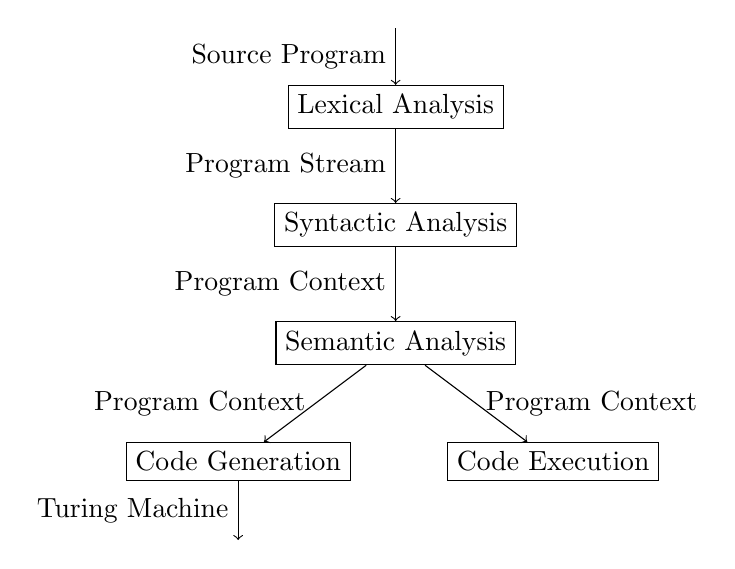
\begin{tikzpicture}
                \node[draw] (CW) at (0, 0) {Lexical Analysis};
                \node[draw] (CP) at (0, -1.5) {Syntactic Analysis};
                \node[draw] (CV) at (0, -3) {Semantic Analysis};
                \node[draw] (CC) at (-2, -4.5) {Code Generation};
                \node[draw] (CE) at (2, -4.5) {Code Execution};
        
                \draw[->] (0, 1) -- node[left] {Source Program} (CW);
                \draw[->] (CW) -- node[left] {Program Stream} (CP);
                \draw[->] (CP) -- node[left] {Program Context} (CV);
                \draw[->] (CV) -- node[left] {Program Context} (CC);
                \draw[->] (CV) -- node[right] {Program Context} (CE);
                \draw[->] (CC) -- node[left] {Turing Machine} (-2, -5.5);
            \end{tikzpicture}
            \caption{The parsing process.}
        \end{figure}
    \end{frame}

    \begin{frame}{Product}
        \begin{enumerate}
            \item Homepage
            \begin{enumerate}
                \item Editor
                \item Convert to FSM and definition
                \item Execute on tape
            \end{enumerate}
            \item Documentation Pages
            \item Error Pages
        \end{enumerate}
        % TODO: DEMO SHOULD BE AROUND THIS TIME
    \end{frame}

    \begin{frame}{Evaluation}
        \begin{itemize}
            \item Unit testing throughout
            \begin{itemize}
                \item Parser
                \item Product- less successful due to mocking
            \end{itemize}
            \item User evaluation- worksheet on TM and TML with second year CS students
            \begin{itemize}
                \item TML was easy to use
                \item Students would consider using TML when constructing TMs
                \item Students believe TML is a good language to learn about TMs while abstracting TM operations
                \item Website is well-designed
            \end{itemize}
            \item A more thorough evaluation would allow us to make stronger conclusions
        \end{itemize}
    \end{frame}

    \begin{frame}{Future Work}
        \begin{itemize}
            \item Improve the language with more features:
            \begin{itemize}
                \item \texttt{move end};
                \item parametrisation.
            \end{itemize}
            \item Make the website more accessible:
            \begin{itemize}
                \item Add a play button;
                \item Make the FSM panel more responsive.
            \end{itemize}
        \end{itemize}
    \end{frame}

    \begin{frame}{Conclusion}
        \begin{itemize}
            \item Project aim- create a PL for TMs and see if it is easier to learn the concept this way.
            \item Constructed the TML, parser for the language and a website to illustrate the parser.
            \item Students believe TML is a good model to plan TM algorithms- abstracts the TM operations well and keeps the tape operations concrete.
            \item A lot of scope for future work, in terms both language and website.
        \end{itemize}
    \end{frame}
    
\end{document}
